\begin{center}
	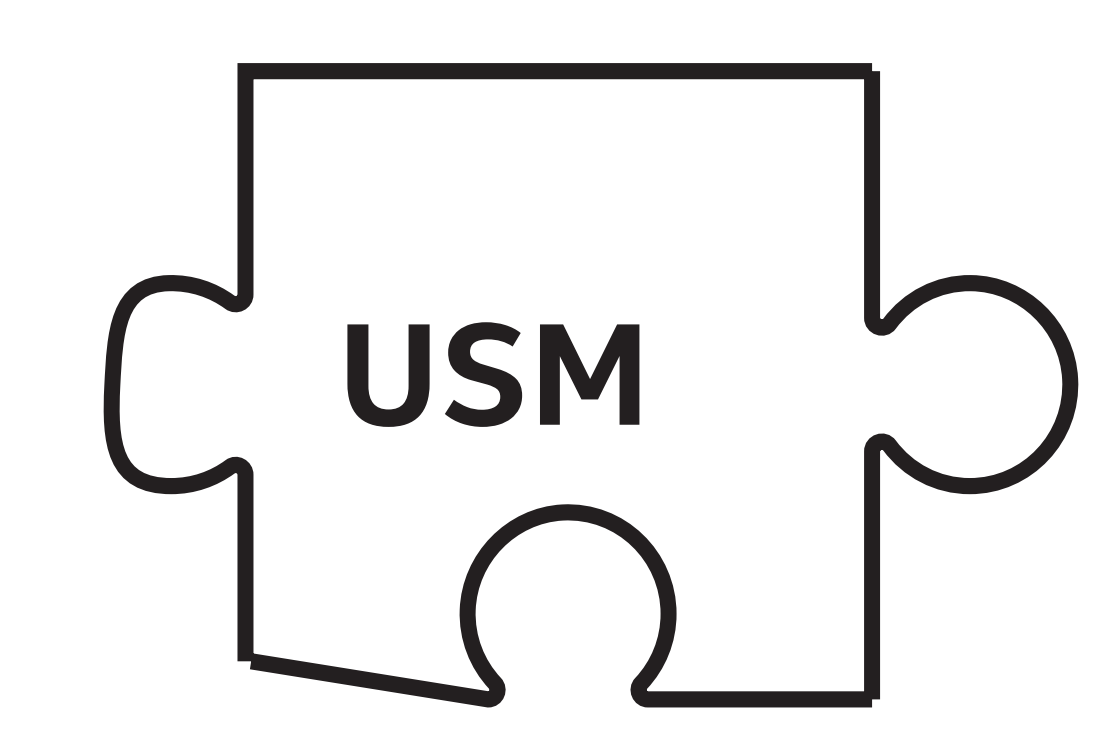
\includegraphics[width=0.3\textwidth]{content/chapter-6/images/1}
\end{center}

接下来的两章将深入探讨如何管理数据。有两种相互补充的方法:统一共享内存(USM)和缓冲区。USM的接口级别与缓冲区不同——USM有指针,而缓冲区使用更高级别的接口。本章主要介绍USM。\par

USM是一个不错的选择,除非我们明确想要使用缓冲区。USM是一种基于指针的内存模型,可以通过指针读写内存。\par